\documentclass{jsarticle}
\usepackage[dvipdfmx]{graphicx}
\usepackage{ascmac} % itemboxを利用するために必要
\usepackage{url}

%図にEPSファイルを採用した場合，PDFファイルが生成されないことがあるので，PNGやJPEG，PDFファイルを図に採用したほうがよい．

\title{ソフトウェア設計及び実験\\前期・個人開発進捗報告書}

\author{学生番号：6125010806　氏名：清水 統貴}
\date{2026年7月1日}

\begin{document}
\maketitle

\section{開発期間2025年6月25日～7月1日の進捗状況}
%

\subsection{前回からの課題と進展事項}
%
現在までにゲームの基盤となる描画ループの構築，コントローラーの入力制御，及び
基礎的な物理演算の実装を完了した．具体的な内容は表\ref{table1}に示す．

\begin{table}[htb]
\begin{center}
\caption{課題と進展}
\label{table1}
\begin{tabular}{|p{7cm}|p{7cm}|}\hline
課題 & 進展 \\ \hline \hline
ウィンドウ描画とメインループの最適化 & SDL2を用いて640×480のウィンドウとレンダラーを生成し，簡単なキャラクターの描画処理を実装した． \\ \hline
Joy-Conによる入力制御と軸変換 & Joy-Con操作に対応するための入力処理を実装した．Joy-Conを横持ちで使用するために，スティックの入力軸の入れ替えを行った． \\ \hline
簡単な物理演算の実装 & 重力については毎フレーム，プレイヤーのY軸方向の速度に対して定数を加算し，それをY軸に反映させることで自然な落下処理を実現した．また，ジャンプボタンを押した際Y軸の上方向に強い初速を与えることで，放物線を描くジャンプを実装した． \\ \hline
\end{tabular}
\end{center}
\end{table}

\begin{figure}[htb]
\centering
\label{figure1}
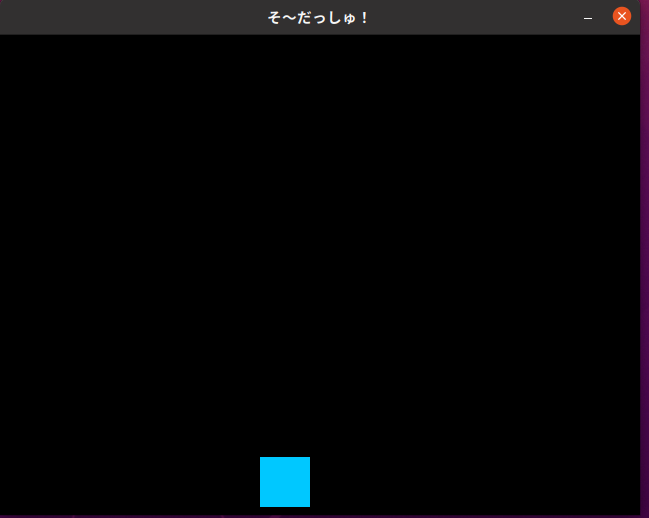
\includegraphics[scale=0.3]{window.png}
\caption{ゲームを実行したときの様子}
\end{figure}

\section{開発期間2026年7月2日～9日の予定}

\subsection{完了させる事項}
企画書のガントチャートに従い，物理演算や移動に関する機能，主にJoy-Conを振ってゲージを溜め，ブースト
する機能の実装を完了させる．

\subsection{新しく取り組む事項}
キャラクターやゲージ，スコア，タイマー等のUIの実装と，それに付随した敵キャラやギミック，
地形の当たり判定の機能の実装もしていきたい．


\begin{thebibliography}{9}
\bibitem{gemini} Google : Gemini \url{https://gemini.google.com/?hl=ja} (2026年7月1日閲覧)
\end{thebibliography}
\end{document}

